\documentclass[11pt,a4paper]{article}

\usepackage{../../templates/style}

\begin{document}

\begin{problem}{SMS Thumb}{standard input}{standard output}{1 second}{1 megabytes}

กำหนดปุ่มกดโทรศัพท์มือถือเป็นดังนี้

\begin{figure}[h!]
\centering
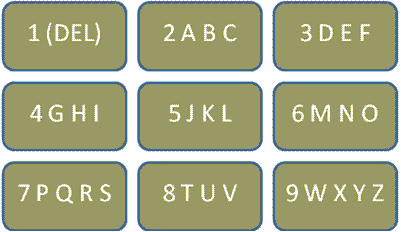
\includegraphics[width=0.6\textwidth]{../latex/img/1059/1059-1.png}
\end{figure}

การกดปุ่มแต่ละครั้งตัวอักษรจะปรากฏวนกันไปตามจำนวนครั้งที่กดตามลำดับ (เฉพาะ ‘A’ - ‘Z’ ไม่มีตัวเลข) ตัวอย่างเช่น การกดปุ่ม \textbf{2} จะปรากฏตัวอักษร \textbf{A B C A B …} วนกันไป ถ้ากดปุ่มนี้จำนวน $5$ ครั้งตัวอักษรที่ได้คือ \textbf{B} และถ้ากดปุ่ม \textbf{7} จำนวน $2$ ครั้งจะได้ตัวอักษร \textbf{Q} เป็นต้น สำหรับปุ่มหมายเลข \textbf{1} จะเป็นการลบตัวอักษรที่พิมพ์ไปก่อนหน้านี้ ครั้งละ $1$ ตัวอักษร หากไม่มีตัวอักษรเหลืออยู่ในข้อความการกดปุ่มนี้จะไม่ส่งผลใดๆ ทั้งสิ้น การเลื่อนนิ้วแต่ละครั้ง (ไปที่ปุ่มใหม่ หรือปุ่มเดิมก็ดี) จะนับเริ่มใหม่ที่ตัวอักษรตัวแรกของปุ่มนั้นเสมอ

 

คาวีสังเกตเห็นนารินกำลังกดปุ่มโทรศัพท์เพื่อส่งข้อความ \textit{SMS} ในพริบตาแรก คาวีเห็นว่านารินเริ่มต้นกดที่ปุ่มไหน ก่อนที่นารินจะรู้ตัวว่าถูกแอบมอง จึงปลีกหลบพ้นสายตาคาวี อย่างไรก็ดีหลังจากนั้นคาวีก็ยังสามารถสังเกตเห็นได้ว่า นารินเลื่อนนิ้วไปทางไหนเพื่อกดปุ่มถัดไป เช่น อยู่ทางซ้าย/ขวา หรือ บน/ล่าง เทียบกับปุ่มปัจจุบันไปกี่ปุ่ม จนกว่านารินจะพิมพ์ข้อความเสร็จ ตัวอย่าง เช่น ถ้าครั้งแรก นารินกดเลข \textbf{8} จำนวน $1$ ครั้ง ซึ่งจะได้ตัวอักษร ‘\textbf{T}’ แล้วเลื่อนนิ้วไปทางขวา $1$ ปุ่ม ขึ้นบน $1$ ปุ่ม และกดปุ่มนั้น $6$ ครั้ง แสดงว่านาริน กดเลข \textbf{6} ซึ่งจะได้ตัวอักษร ‘\textbf{O}’ ดังนั้นข้อความที่นารินกดอ่านได้เป็น “\textbf{TO}” จากแฟ้มข้อมูลการพิมพ์ \textit{SMS} ที่คาวีสังเกตเห็น (นารินไม่เลื่อนนิ้วออกนอกแป้นตัวเลขเลย)

\bigskip
\underline{\textbf{โจทย์}}  จงเขียนโปรแกรมหาข้อความที่นารินพิมพ์

\InputFile

\textbf{บรรทัดแรก} รับจำนวนครั้งที่เลือกปุ่มกด $N$ $(1 \leq N \leq 80)$ จนพิมพ์ข้อความเสร็จ

\textbf{บรรทัดที่สอง} รับข้อมูลปุ่มแรกที่เลือกกด $S$ $(1 \leq S \leq 9)$ และจำนวนครั้งที่กด $M$ $(1 \leq M \leq 4\,096)$ คั่นด้วยช่องว่าง

\textbf{บรรทัดที่ $3$ ถึง $N+2$} ในบรรทัดที่ $i+1$ ให้รับข้อมูลการเลือกปุ้มครั้งที่ $i$ แต่ละบรรทัดจะประกอบด้วยตัวเลข $3$ จำนวน จำนวนแรก แสดงทิศทางแนวนอน $H$ จากปุ่มที่กดก่อนหน้านี้ จำนวนที่สอง แสดงทิศทางแนวตั้ง $V$ จากปุ่มที่กดก่อนหน้านี้ และจำนวนที่สาม แสดงจำนวนครั้งที่กดปุ่มนั้น ($M_i$) โดยจำนวนทั้งสามจะคั่นด้วยช่องว่าง

ข้อมูลของการเคลื่อนปุ่มมีดังนี้:
\begin{itemize}

\item ทิศทางแนวนอน $H$ อยุ้ในเซต $\{ –2, –1, 0, 1, 2 \}$ โดยจำนวนลบแสดงการเลื่อนไป ทางซ้าย และจำนวนบวกแสดงการเลื่อนไป ทางขวา
\item ทิศทางแนวตั้ง V อยู่ในเซต $\{ –2, –1, 0, 1, 2 \}$ โดยจำนวนลบแสดงการเลื่อน ขึ้นบน และจำนวนบวกแสดงการเลื่อน ลงล่าง
\item ค่าสัมบูรณ์ของตัวเลข แสดงจำนวนปุ่มที่เลื่อนไปในทิศทางนั้นๆ ดังนั้น เลข 0 หมายถึงไม่มีการเลื่อนในแนวนั้น
\end{itemize}

\OutputFile

\textbf{บรรทัดเดียว} แสดงสตริงข้อความที่พิมพ์ (ไม่มีการเว้นช่องว่าง) ถ้าไม่ได้พิมพ์อะไรเลยให้แสดงคำว่า null 

\Examples

\begin{example}
\exmp{4
5 3
1 0 3
-1 1 3
1 -2 2}{LOVE}%
\exmp{2
9 6
-2 -2 5	}{null}%
\exmp{5
3 3
0 0 2
-2 0 1
2 1 3
0 1 2}{FOX}%
\end{example}


\Source

การแข่งขันคอมพิวเตอร์โอลิมปิกสอวน.ครั้งที่ 4 ปี 2551 วันที่ 1

\end{problem}

\end{document}